%This is part of Un soupçon de mathématique sans être agressif pour autant
% Copyright (c) 2012-2013
%   Laurent Claessens, Pauline Klein
% See the file fdl-1.3.txt for copying conditions.

%+++++++++++++++++++++++++++++++++++++++++++++++++++++++++++++++++++++++++++++++++++++++++++++++++++++++++++++++++++++++++++
\section{Introduction}
%+++++++++++++++++++++++++++++++++++++++++++++++++++++++++++++++++++++++++++++++++++++++++++++++++++++++++++++++++++++++++++

\begin{Aprojeter}
    \begin{example} \label{ExemVmCkIH}
        Un petit tour de magie. Choisissez un nombre entre \( 1\) et \( 10\). Ajoutez \( 5\), multipliez par \( 2\), ajoutez \( 7\), enlevez le double du nombre de départ.
    \end{example}
\end{Aprojeter}

\begin{Aprojeter}
    Pouvez-vous trouver un petit tour de magie qui commence par
    \begin{itemize}
        \item Multiplier par \( 3\)
        \item Faire \( +2\)
        \item \ldots
    \end{itemize}
    et qui donne toujours \( 5\) ?
\end{Aprojeter}

\begin{Aprojeter}
    \lstinputlisting{ex_algo18.py}
\end{Aprojeter}

%+++++++++++++++++++++++++++++++++++++++++++++++++++++++++++++++++++++++++++++++++++++++++++++++++++++++++++++++++++++++++++
\section{Courbe représentative d'une fonction}
%+++++++++++++++++++++++++++++++++++++++++++++++++++++++++++++++++++++++++++++++++++++++++++++++++++++++++++++++++++++++++++

%TODO : il faut essayer de refaire une figure pour tous les dessins de Pauline.
Soit $f$ une fonction définie sur un ensemble $\defD$.

\begin{definition}
    On appelle \defe{représentation graphique}{représentation graphique (d'une fonction)}, ou le \defe{graphe}{graphe} de $f$, l'ensemble des points $(x,y)$ tels que $x\in\defD$ et $y=f(x)$.
\end{definition}


\begin{Aprojeter}



\begin{Aretenir}
    La règle d'or des graphiques : le point de coordonnées \( (a;b)\) est sur le graphique de la fonction \( f\) si et seulement si \( f(a)=b\).
\end{Aretenir}

%The result is on figure \ref{LabelFigAHAbqhj}. % From file AHAbqhj
%\newcommand{\CaptionFigAHAbqhj}{<+Type your caption here+>}
%\input{Fig_AHAbqhj.pstricks}

%\begin{wrapfigure}{r}{7.0cm}
%   \vspace{-0.5cm}        % à adapter.
%   \centering

À propos du graphe suivant :
\begin{center}
   \input{Fig_AHAbqhj.pstricks}
\end{center}
%\end{wrapfigure}
\begin{enumerate}
    \item
        Quel est l'ensemble de définition de la fonction \( f\) ?
    \item
        Quelle est l'image de \( 1\) par \( f\) ?
    \item
        Donner un antécédent de \( 3\).
    \item
        Quels sont les antécédents de \( -1\) ?
\end{enumerate}
    
\end{Aprojeter}

\begin{example}
    Soit la fonction \( f(x)=3x-1\).
    \begin{enumerate}
        \item
            Le point \( (0;-1)\) est sur la courbe représentative de \( f\) parce que \( f(0)=1\).
        \item
            Le point \( (10;29)\) est également sur la courbe parce que \( f(10)=29\).
        \item
            Le point \( (2;3)\) n'est par contre pas sur le graphe parce que \( f(2)=5\neq 4\).
    \end{enumerate}
\end{example}

Quelque conseils pour dessiner.
\begin{itemize}
    \item
        Pour une valeur $x$ sur l'axe des abscisses, il y a un et un seul point d'abscisse $x$ sur la courbe.
    \item
        Pour tracer une courbe, il faut placer des points. Plus on choisit de points, plus la courbe sera précise.
    \item
        Si possible, trouver quelque valeurs clefs. Par exemple on cherchera les points d'intersection entre les axes et les courbe. Le point \( (0,f(0)) \) est intéressant à mettre, ainsi que les points \( x\) tels que \( f(x)=0\).
\end{itemize}

\begin{example}
    Créons un petit programme définissant la fonction \( f(x)=x^2-2\) et en calculant \( 10\) valeurs régulièrement espacées entre \( -5\) et \( 5\). La production d'une liste de nombre régulièrement espacés est un travail pour la fonction \info{numpy.linspace}. La syntaxe en est 
\begin{quote}
    \info{numpy.linspace(a,b,num=n)}
\end{quote}
Cela est une liste de \info{n} nombres régulièrement espacés entre \info{a} et \info{b}. En ce qui concerne le carré, en python les puissances sont données par \info{**}. Par exemple \info{a**3} est le cube de \info{a} :
\begin{verbatim}
>>> 2**3
8
\end{verbatim}
Le programme est

\lstinputlisting{ex_graphe.py}

Le programme donne :

%\lstinputlisting[title=Résultat]{res_ex_graphe.txt}

\VerbatimInput{res_ex_graphe.txt}
    
\end{example}



\newcommand{\CaptionFigExFonction}{Comment tracer la fonction \( f\colon x\to 2x+1\) ?}
\input{Fig_ExFonction.pstricks}

Nous donnons à la figure \ref{LabelFigExFonction} le tracé de la fonction \( f(x)=2x+1\). La figure \ref{LabelFigExFonctionssLabelSubFigExFonction0} donne quelque points du graphe de la fonction. La figure \ref{LabelFigExFonctionssLabelSubFigExFonction1} donne le graphe complet de la fonction. Comment le construit-on ? Par définition pour chaque \( x\) sur l'axe des abscisses (il y en a une infinité), il faut calculer le nombre \( f(x)\) et mettre dans le plan le point de coordonnées \( \big( x,f(x) \big)\).

En pratique, il n'est pas possible de calculer \( f(x)\) pour \emph{tous} les \( x\) réels\footnote{Chuck Norris peut le faire.}. C'est pourquoi nous nous contentons qu'en calculer quelque uns, et nous les relions «le plus intelligemment possible».



%---------------------------------------------------------------------------------------------------------------------------
\subsection{Ce qui n'est pas une fonction}
%---------------------------------------------------------------------------------------------------------------------------

%    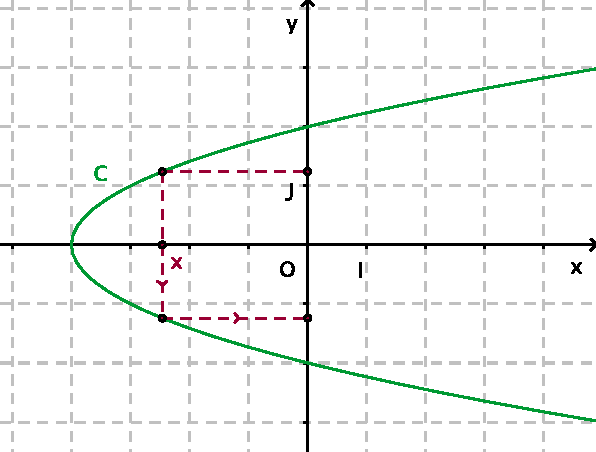
\includegraphics[width=5cm]{F_NonFct.pdf}

\begin{multicols}{2}
    Cette courbe ne représente pas une fonction, car à partir de \( x=-4\), les nombres ont deux images. Les courbes données par des fonctions sont des courbes acceptant une seule ordonnée pour chaque abscisse.

\columnbreak

%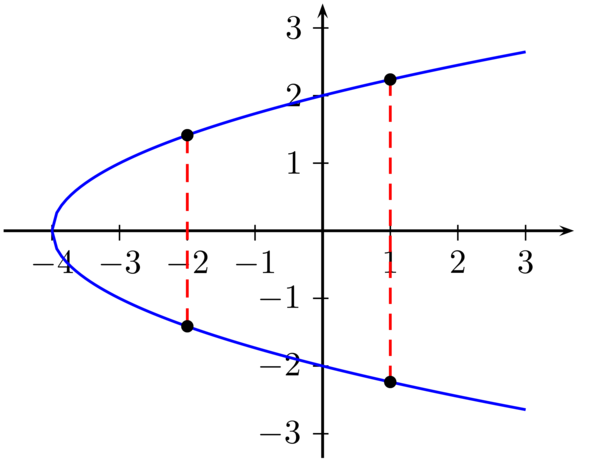
\includegraphics{Picture_FIGLabelFigPasFonctionYoQfSuPICTPasFonctionYoQfSu-for_eps.pdf}

\input{Fig_PasFonctionYoQfSu.pstricks}

\end{multicols}


%+++++++++++++++++++++++++++++++++++++++++++++++++++++++++++++++++++++++++++++++++++++++++++++++++++++++++++++++++++++++++++ 
\section{Ensemble de définition}
%+++++++++++++++++++++++++++++++++++++++++++++++++++++++++++++++++++++++++++++++++++++++++++++++++++++++++++++++++++++++++++

\begin{definition}
    Soit \( \defD\) un ensemble de nombres. On définit une \defe{fonction}{fonction} \( f\) sur \( \defD\) en associant à chaque nombre \( x\) dans \( \defD\) un seul nombre \( y\). Dans ce cas nous disons que \( f\) est une fonction de la \defe{variable}{variable} \( x\).
\end{definition}

\begin{example}
    Soit la fonction qui à la longueur d'un segment fait correspondre la surface du carré construit sur ce segment. Cette fonction n'est définie que sur les nombres positifs (parce qu'il n'existe pas de segments de longueurs négatives). Nous écrivons donc
    \begin{equation}
        \begin{aligned}
            f\colon \mathopen[ 0 , \infty [&\to \eR \\
            x&\mapsto x^2,
        \end{aligned}
    \end{equation}
    et nous avons \( f(x)=x^2\).

    Le symbole \( \mathopen[ 0 , \infty [\) représente l'ensemble de tous les nombres de \( 0\) (y compris) à l'infini, c'est à dire tous les nombres plus grands ou égaux à \( 0\).
\end{example}

\begin{example}
    Soit la fonction qui a un nombre entier fait correspondre la somme de ses chiffres. Par exemple \( f(0)=0\) et \( f(123)=6\). Cette fonction est définie sur les entiers et retourne un entier. Nous pouvons écrire
    \begin{equation}
        \begin{aligned}
            f\colon \eN&\to \eN \\
            x&\mapsto f(x). 
        \end{aligned}
    \end{equation}
    Ici il est compliqué de donner une forme explicite pour \( f\).
\end{example}

\begin{example}
    La fonction carré est :
    \begin{equation}
        \begin{aligned}
            f\colon \eR&\to \eR \\
            x&\mapsto x^2 
        \end{aligned}
    \end{equation}
    Notons que c'est presque la même que la fonction «surface du carré». La différence est le contexte.
\end{example}

\begin{example}
    La fonction racine carré est :
    \begin{equation}
        \begin{aligned}
            \sqrt{}\colon \mathopen[ 0 , \infty [&\to \eR  \\
                x&\mapsto \sqrt{x}. 
        \end{aligned}
    \end{equation}
\end{example}

\begin{example}
    La fonction inverse est :
    \begin{equation}
        \begin{aligned}
            f\colon \eR\setminus\{ 0 \}&\to \eR \\
            x&\mapsto \frac{1}{ x }. 
        \end{aligned}
    \end{equation}
    La notation \( \eR\setminus\{ 0 \}\) représente l'ensemble de tous les nombres sauf zéro.
\end{example}

%--------------------------------------------------------------------------------------------------------------------------- 
\subsection{Intermède : pourquoi ne pas diviser par zéro ?}
%---------------------------------------------------------------------------------------------------------------------------

La fraction \( \frac{1}{ 0.1 }\) est le nombre de fois que \( 0.1\) rentre dans \( 1\). Cela vaut \( 10\) parce qu'il faut \( 10\) soit \( 0.1\) pour faire \( 1\).

Que vaut \( \frac{1}{ 0.0001 }\) ? C'est le nombre de fois que \( 0.0001\) rentre dans \( 1\), c'est à dire dix mille.

Que vaudrait \( \frac{1}{ 0 }\) ? C'est le nombre de fois qu'il faut prendre zéro pour obtenir \( 1\).

\begin{example}
    Considérons la fonction qui a un nombre fait correspondre son inverse : \( f\colon x\mapsto \frac{1}{ x }\). Pour se dérouiller le cerveau, je propose quelque valeurs :
    \begin{equation}
        \begin{aligned}[]
            f(1)&=1&f(5)&=\frac{1}{ 5 }&f(\frac{ 2 }{ 3 })=\frac{ 3 }{ 2 }\\
            f(\frac{ 1 }{ 4 })&=4&f(-3)&=-\frac{1}{ 3 }&f(-1)&=-1.
        \end{aligned}
    \end{equation}
    Cette fonction est implémentée en python de la façon suivante :

\lstinputlisting{ex_inverse.py}

donne

%\lstinputlisting[title=Résultat]{res_ex_inverse.txt}
\VerbatimInput{res_ex_inverse.txt}

Très clairement, python ne veut pas calculer l'inverse de zéro et plante sur un message on ne peut plus clair : \info{ZeroDivisionError: division by zero}.

Effectivement, l'inverse de zéro n'existe pas. L'ensemble de définition de notre fonction \( f(x)=1/x\) n'est donc pas \( \eR\) tout entier, mais seulement \( \eR\setminus\{ 0 \}\).

\end{example}

\begin{Aretenir}        \label{ArtJgipNt}
    Il n'est pas permis de diviser par zéro. Une fonction qui contient un dénominateur ne peut pas avoir dans son ensemble de définition des \( x\) qui annulent le dénominateur. Autrement dit dès que vous voyez
    \begin{equation}
        \frac{1}{ f(x) }
    \end{equation}
    vous devez résoudre l'équation \( f(x)=0\).
\end{Aretenir}

%+++++++++++++++++++++++++++++++++++++++++++++++++++++++++++++++++++++++++++++++++++++++++++++++++++++++++++++++++++++++++++
\section{Antécédent}
%+++++++++++++++++++++++++++++++++++++++++++++++++++++++++++++++++++++++++++++++++++++++++++++++++++++++++++++++++++++++++++

\begin{Aretenir}
Une fonction associe à chaque nombre de l'ensemble de définition \emph{un seul} nombre, appelé \defe{image}{image}. Si \( a\) est un nombre, un \defe{antécédent}{antécédent} de \( a\) par la fonction \( f\) est un nombre \( x\in\defD\) tel que 
\begin{equation}
    f(x)=a.
\end{equation}
Autrement dit, les antécédents de \( a\) sont les éléments de \( \eR\) dont l'image par \( f\) est \( a\).

Il peut arriver qu'un nombre ait plusieurs antécédents.
\end{Aretenir}


\begin{example}
    Pour la fonction \( f(x)=2x-1\), un antécédent de \( 5\) est le nombre \( 3\). Un antécédent du nombre \( -10\) est la nombre \( -9/2\).
\end{example}

\begin{Aretenir}
    Trouver les antécédents de \( a\) par la fonction \( f\) revient à trouver les solutions de l'équation
    \begin{equation}
        f(x)=a.
    \end{equation}
\end{Aretenir}


\begin{example}

    Les antécédents de \( 4\) pour la fonction \( f(x)=2x-1\) sont les solutions de l'équation
    \begin{equation}
        2x-1=4
    \end{equation}
    c'est à dire \( x=\frac{ 5 }{2}\). Il se fait qu'il y en a un seul.

    Plus généralement l'antécédent de \( a\) pour cette fonction est la solution de l'équation
    \begin{equation}
        2x-1=a,
    \end{equation}
    c'est à dire le nombre \( x=\frac{ a+1 }{ 2 }\).
\end{example}

\begin{example} \label{EqlaIGDz}
    Si nous avons une série statistique de \( n\) valeurs, pour trouver le premier quartile nous devons diviser \( n\) par \( 4\) et prendre l'entier le plus proche vers le haut. Cela donne le numéro de la valeur correspondante au premier quartile.

    En python, la fonction qui donne le numéro de la valeur du premier quartile en fonction de \( n\) est
    \begin{quote}
        \info{math.ceil(n/4)}
    \end{quote}
    Notons \( f\) cette fonction. Son ensemble de définition est l'ensemble des entiers non nuls. Le graphique de cette fonction est donné à la figure \ref{LabelFigMathCeilwCXIJZ}.
\newcommand{\CaptionFigMathCeilwCXIJZ}{Le numéro de la valeur du premier quartile en fonction du nombre de valeurs.}
\input{Fig_MathCeilwCXIJZ.pstricks}

    Le graphique est uniquement constitué de points. Pas de lignes entre, parce qu'il n'existe pas de séries statistiques comprenant \( 3.7\) valeurs par exemple. 
\end{example}

\Exo{Seconde-0053}

\begin{example}
    Soit la fonction définie sur \( \defD=\{ -5,-1,1,3,9 \}\) de la façon suivante :
    \begin{equation}
        \begin{array}[h]{|c||c|c|c|c|c|c|}
            \hline
            x&-5&-1&1&3&9&10\\
            \hline
            f(x)&0&2&-3&7&2&5\\
            \hline
        \end{array}
    \end{equation}
    Nous pouvons dire que
    \begin{enumerate}
        \item
            L'image de \( 1\) par \( f\) est \( -3\).
        \item
            L'unique antécédent de \( 7\) est \( 3\).
        \item
            Les nombres \( -1\) et \( 9\) sont tous deux des antécédents de \( 2\).
    \end{enumerate}
\end{example}

\begin{example}
    Soit la fonction \( f(x)=(x+1)^2\). Nous avons \( f(-1)=0\), \( f(4)=25\); nous disons que \( 0\) est l'image de \( -1\) par \( f\) et que \( 25\) est l'image de \( 4\) par \( f\).

    Remarquons que \( f(-2)=1\) et \( f(0)=1\). Donc \( -2\) et \( 0\) sont deux antécédents de \( 1\).
\end{example}

\begin{example}
    Le nombre \( 4\) est un antécédent de \( 3\) pour la fonction \( f(x)=\frac{ x }{ 2 }+1\).
\end{example}

\begin{example}
    Les nombres \( 3\) et \( -3\) sont tout deux des antécédents de \( 9\) pour la fonction \( x\mapsto x^2\).
\end{example}

%+++++++++++++++++++++++++++++++++++++++++++++++++++++++++++++++++++++++++++++++++++++++++++++++++++++++++++++++++++++++++++
\section{Modélisation par une fonction}
%+++++++++++++++++++++++++++++++++++++++++++++++++++++++++++++++++++++++++++++++++++++++++++++++++++++++++++++++++++++++++++

Les exemples de fonctions dans la «vraie» vie sont nombreux.

\begin{example}
    Soit un triangle rectangle isocèle dont les côtés de l'angle droit sont de longueur \( x\). Alors la surface est donnée par la fonction
    \begin{equation}
        f(x)=\frac{ x^2 }{2}.
    \end{equation}
    L'ensemble de définition est \( \defD=\mathopen] 0 , \infty \mathclose[\) parce que \( x\) représente une longueur.
\end{example}

\begin{example}
    Un vélo se déplace à \( \unit{20}{\kilo\meter\per\hour}\). Après un temps \( t\), il aura parcouru une distance
    \begin{equation}
        d(t)=20t
    \end{equation}
    kilomètres. Ici l'ensemble de définition est plus délicat; il dépend du contexte.

    Notons que la variable d'une fonction n'est pas obligatoirement toujours notée \( x\) et que la fonction n'est pas toujours obligatoirement notée \( f\).
\end{example}

\begin{example}
    Vous verrez dans un cours de physique que si on lance un objet verticalement avec une vitesse initiale \( v_0\), alors la hauteur en fonction du temps est donnée par
    \begin{equation}
        h(t)=v_0t-\frac{ gt^2 }{2}
    \end{equation}
    où \( g\) est l'accélération de la gravitation sur Terre (environ \( \unit{10}{\meter\per\second\squared}\)).
\end{example}

